\documentclass[12pt,a4paper]{article}

\usepackage[T1]{fontenc}
\usepackage[utf8]{inputenc}
\usepackage[a4paper, margin=2.5cm]{geometry}
\usepackage{amsmath}
\usepackage{amssymb}
\usepackage{graphicx}
\usepackage{hyperref}
\usepackage{listings}
\usepackage{xcolor}
\usepackage{tikz}
\usepackage{booktabs}
\usepackage{array}
\usepackage{parskip}
\usepackage{microtype}
\usepackage{enumitem}
\usepackage{float}
\usepackage{caption}
\usepackage{subcaption}
\usetikzlibrary{shapes.geometric, arrows.meta, positioning, fit, backgrounds}

\hypersetup{
  colorlinks=true,
  linkcolor=blue!60!black,
  citecolor=green!50!black,
  urlcolor=blue!70!black,
  pdfauthor={},
  pdftitle={FunAutoScripter: Automatic Funscript Generation via Classical Optical Flow},
}

% Listings style for Python snippets
\lstdefinestyle{pysnip}{
  language=Python,
  basicstyle=\ttfamily\small,
  keywordstyle=\bfseries\color{blue!70!black},
  commentstyle=\itshape\color{gray},
  stringstyle=\color{green!50!black},
  showstringspaces=false,
  frame=single,
  framerule=0.4pt,
  rulecolor=\color{black!20},
  backgroundcolor=\color{black!3},
  xleftmargin=1em,
  xrightmargin=1em,
  aboveskip=0.7em,
  belowskip=0.7em,
  numbers=none,
  breaklines=true,
}

% JSON / funscript snippet style
\lstdefinestyle{jsonsnip}{
  basicstyle=\ttfamily\small,
  showstringspaces=false,
  frame=single,
  framerule=0.4pt,
  rulecolor=\color{black!20},
  backgroundcolor=\color{black!3},
  xleftmargin=1em,
  xrightmargin=1em,
  aboveskip=0.7em,
  belowskip=0.7em,
  numbers=none,
  breaklines=true,
}

\title{\textbf{FunAutoScripter}\\[0.4em]
  \large Automatic Funscript Generation from Video\\
  using Classical Optical Flow}
\author{}
\date{October 2026}

\begin{document}

\maketitle
\thispagestyle{empty}

\begin{abstract}
FunAutoScripter is a command-line and graphical tool that automatically
generates \emph{funscripts} --- synchronisation files for linear actuator
devices --- directly from video, without human annotation and without any
neural network or machine-learning model. The tool decodes video with ffmpeg,
computes dense optical flow (Farneback algorithm) on a downsampled greyscale
stream, selects the region of interest with a periodicity-weighted score,
projects flow onto a dominant motion axis derived by PCA, integrates to a
position signal, applies a Butterworth bandpass filter, normalises with a
rolling-window percentile, and finally extracts peaks and valleys as keyframes
with a speed constraint. The entire pipeline is classical signal processing;
the only runtime dependencies are numpy, scipy, OpenCV and ffmpeg. On synthetic
test videos the output achieves Pearson correlation coefficients of 0.97--0.99
with ground-truth motion, and the system detects scene cuts with millisecond
precision through a dual absolute/relative threshold test on frame-difference
spikes.
\end{abstract}

\tableofcontents
\clearpage

%% ============================================================
\section{Introduction}
\label{sec:intro}
%% ============================================================

\subsection{Funscripts and linear actuator devices}

A funscript is a JSON file that encodes a time-stamped sequence of position
commands for a motorised stroker device. Each \emph{action} is a pair
\(\{\texttt{at}: t,\; \texttt{pos}: p\}\) where \(t\) is a timestamp in
milliseconds and \(p \in [0, 100]\) is the target position (0 = fully
retracted, 100 = fully extended). The device firmware interpolates linearly
between consecutive actions, so the speed of a stroke is determined by
\(\Delta p / \Delta t\). A minimal funscript looks like:

\begin{lstlisting}[style=jsonsnip]
{
  "version": "1.0",
  "inverted": false,
  "range": 90,
  "actions": [
    {"at": 1200, "pos": 0},
    {"at": 1650, "pos": 100},
    {"at": 2100, "pos": 0}
  ]
}
\end{lstlisting}

Creating such files by hand --- watching a video and clicking for each stroke
--- is accurate but extremely tedious, typically taking several times the
length of the video to script. The community has produced semi-automated tools,
but most require either deep-learning models with GPU requirements or
substantial manual interaction.

\subsection{Motivation and scope}

FunAutoScripter targets the case where the motion in the video is directly
observable as optical flow: a region of the frame oscillates periodically along
a dominant axis, and the amplitude and timing of that oscillation should drive
the device. No semantic understanding of the scene is needed; only spatiotemporal
analysis of pixel displacements.

Design constraints were strict:
\begin{itemize}[nosep]
  \item No neural networks, no ONNX models, no PyTorch, no YOLO --- ever.
  \item CPU only; must produce results in reasonable time without a GPU.
  \item Minimal dependencies: numpy, scipy, OpenCV, matplotlib (for
    diagnostics only), system ffmpeg. The optional GUI adds DearPyGui.
  \item Runs correctly inside NixOS \texttt{nix-shell}; no global
    \texttt{pip install}.
\end{itemize}

%% ============================================================
\section{System Architecture}
\label{sec:arch}
%% ============================================================

\subsection{Module structure}

The repository is split into a thin CLI entry point
(\texttt{funautoscripter.py}), an optional GUI entry point
(\texttt{funautoscripter\_gui.py}), and an engine in \texttt{src/}:

\medskip
\begin{center}
\begin{tabular}{@{}ll@{}}
\toprule
Module & Responsibility \\
\midrule
\texttt{src/flow.py}      & ffmpeg decode, Farneback optical flow, disk cache \\
\texttt{src/roi.py}       & region-of-interest selection, axis estimation \\
\texttt{src/signal.py}    & velocity, integration, bandpass, normalisation, keyframes \\
\texttt{src/output.py}    & write funscript JSON, produce debug plots \\
\texttt{src/debug.py}     & annotated diagnostic video generation \\
\texttt{src/chapters.py}  & chapter management and automatic detection \\
\texttt{src/pipeline.py}  & top-level \texttt{process()}, argument parser \\
\texttt{src/gui/app.py}   & DearPyGui application (\texttt{App} class) \\
\texttt{src/gui/config.py}& constants, parameter definitions, themes, built-in presets \\
\texttt{src/gui/utils.py} & colour helpers, path utilities, config I/O \\
\texttt{src/gui/frame\_source.py} & \texttt{FrameSource}: OpenCV video-capture wrapper \\
\bottomrule
\end{tabular}
\end{center}

\subsection{Data-flow overview}

Figure~\ref{fig:pipeline} shows the linear data flow from video to funscript.
Steps 2--7 are all performed in memory in milliseconds; only step 1
(optical flow) is computationally expensive and is therefore cached.

\begin{figure}[H]
\centering
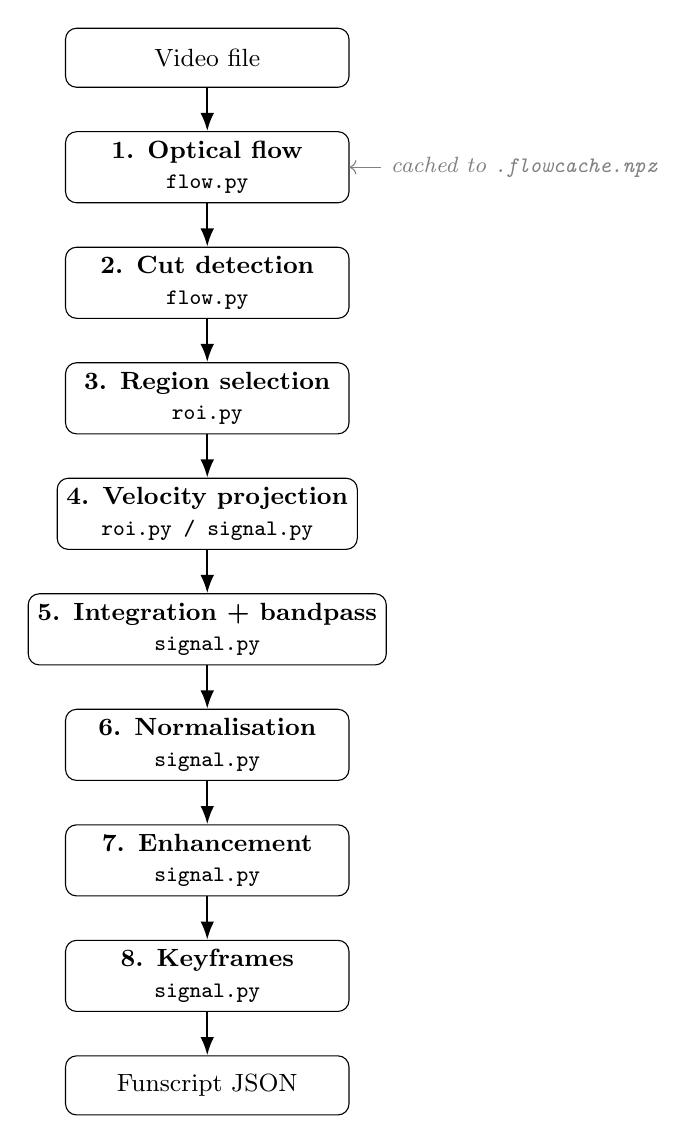
\begin{tikzpicture}[
  box/.style={rectangle, draw, rounded corners=4pt,
              minimum width=3.6cm, minimum height=0.75cm,
              align=center, font=\small},
  arr/.style={-Latex, thick},
  note/.style={font=\footnotesize\itshape, text=gray},
  every node/.style={},
]
  \node[box] (vid)  {Video file};
  \node[box, below=0.55cm of vid]  (flow) {\textbf{1. Optical flow}\\\footnotesize \texttt{flow.py}};
  \node[box, below=0.55cm of flow] (cut)  {\textbf{2. Cut detection}\\\footnotesize \texttt{flow.py}};
  \node[box, below=0.55cm of cut]  (roi)  {\textbf{3. Region selection}\\\footnotesize \texttt{roi.py}};
  \node[box, below=0.55cm of roi]  (vel)  {\textbf{4. Velocity projection}\\\footnotesize \texttt{roi.py / signal.py}};
  \node[box, below=0.55cm of vel]  (int)  {\textbf{5. Integration + bandpass}\\\footnotesize \texttt{signal.py}};
  \node[box, below=0.55cm of int]  (nrm)  {\textbf{6. Normalisation}\\\footnotesize \texttt{signal.py}};
  \node[box, below=0.55cm of nrm]  (enh)  {\textbf{7. Enhancement}\\\footnotesize \texttt{signal.py}};
  \node[box, below=0.55cm of enh]  (kf)   {\textbf{8. Keyframes}\\\footnotesize \texttt{signal.py}};
  \node[box, below=0.55cm of kf]   (out)  {Funscript JSON};

  \foreach \a/\b in {vid/flow, flow/cut, cut/roi, roi/vel, vel/int, int/nrm,
                     nrm/enh, enh/kf, kf/out}
    \draw[arr] (\a) -- (\b);

  % Cache annotation
  \node[note, right=0.4cm of flow] (cn) {cached to \texttt{.flowcache.npz}};
  \draw[->, gray, thin] (cn.west) -- +(-0.3,0) |- (flow.east);
\end{tikzpicture}
\caption{Eight-step pipeline from video file to funscript JSON. Only step 1
(optical flow) is slow; the cache makes repeated runs with different parameters
instantaneous.}
\label{fig:pipeline}
\end{figure}

%% ============================================================
\section{Pipeline}
\label{sec:pipeline}
%% ============================================================

\subsection{Step 1 --- Optical flow extraction}
\label{sec:flow}

The video is decoded by ffmpeg to raw greyscale frames at a fixed resolution
(\texttt{--width}, default 192~px) and frame rate (\texttt{--fps}, default
30~fps). Decoding at reduced resolution is intentional: at 192~px a
1280-pixel-wide frame is compressed by factor 6.7, which reduces noise from
compression artefacts and makes Farneback tractable on a CPU.

Dense optical flow between consecutive greyscale frames
$I_t$ and $I_{t+1}$ is computed with the Farneback algorithm
\cite{farneback2003} as implemented in OpenCV:
\begin{equation}
  \mathbf{f}_t(x,y) = \begin{pmatrix} u_t(x,y) \\ v_t(x,y) \end{pmatrix}
  \approx \arg\min_{\mathbf{f}}
    \int_\Omega \!\bigl\|\nabla I_t \cdot \mathbf{f} + I_t - I_{t+1}\bigr\|^2
    w(\mathbf{x})\,d\mathbf{x}
\end{equation}
where $w$ is a Gaussian weighting window. The result is a per-pixel
displacement field $(u_t, v_t)$ in pixel units.

The per-pixel fields are then spatially averaged over non-overlapping cells of
side \texttt{--cell} (default 12~px), producing three three-dimensional arrays:
\begin{equation}
  \mathrm{dx}[t, g_y, g_x],\quad
  \mathrm{dy}[t, g_y, g_x],\quad
  \mathrm{mag}[t, g_y, g_x]
  = \sqrt{\mathrm{dx}^2 + \mathrm{dy}^2}
\end{equation}
indexed by frame $t$ and grid cell $(g_y, g_x)$. The mean absolute
frame-to-frame difference \texttt{diff}$[t]$ is also stored; it drives cut
detection in the next step.

The result is stored in \texttt{<output>.flowcache.npz}. The cache key encodes
every parameter that affects step~1 (resolution, cell size, fps, crop, zoom,
hardware-acceleration flags and a \texttt{CACHE\_VERSION} integer), so a stale
cache is never silently reused.

\paragraph{Hardware acceleration.}
\texttt{--hwaccel} passes \texttt{-hwaccel auto} to ffmpeg for hardware-assisted
decode. \texttt{--opencl} uses \texttt{cv2.UMat} to offload Farneback to an
OpenCL device; when no GPU is found it falls back to CPU with a diagnostic
message. Parallel flow extraction (\texttt{--jobs~N}) splits the video into
chunks $\geq 20$~s processed in Python threads; OpenCV releases the GIL during
Farneback, so true parallelism is achieved. On a 2-core machine this raised
throughput from 172~fps to 300~fps on a test video.

\paragraph{Zoom for subtle motion.}
At 192~px width, a 1-pixel camera-space displacement becomes 0.15~px in the
analysis grid, which is close to Farneback noise (Table~\ref{tab:zoom}).
\texttt{--zoom X0:Y0:X1:Y1} (normalised frame fractions) crops the motion zone
\emph{before} downsampling, so the 192~px budget is spent entirely on the
region of interest. The zoom factor in the experiment was 3.7$\times$; at 1~px
motion in the original this improved correlation from 0.29 to 0.73.

\begin{table}[H]
\centering
\caption{Correlation of generated script with ground-truth motion for a
1.2~Hz oscillating square at low contrast (30/255) and heavy compression
(CRF~28), as a function of pixel displacement and analysis configuration.
\texttt{--zoom} used a 3.7$\times$ crop.}
\label{tab:zoom}
\small
\begin{tabular}{@{}lccccccc@{}}
\toprule
Motion (px) & Analysis (px) & 192~px & \texttt{--noise 0.01} &
  \texttt{--width 384} & \texttt{--width 768} & \texttt{--zoom} &
  \texttt{--zoom} + noise \\
\midrule
2   & 0.30 & 0.86 & 0.91 & 0.92 & 0.89 & 0.92 & 0.92 \\
1   & 0.15 & 0.29 & 0.46 & 0.55 & 0.61 & 0.73 & 0.77 \\
0.5 & 0.075 & 0.07 & 0.10 & 0.00 & 0.04 & 0.13 & 0.17 \\
\bottomrule
\end{tabular}
\end{table}

\subsection{Step 2 --- Scene cut detection}
\label{sec:cuts}

Each scene boundary resets the region selection, velocity direction and
normalisation, so accurate cut detection is essential. The function
\texttt{detect\_cuts()} uses a dual-threshold strategy on the
frame-difference signal \texttt{diff}$[t]$.

A frame is marked as a cut if \emph{either} condition holds:
\begin{align}
  \texttt{diff}[t] &> \tau_\mathrm{abs} \tag{absolute} \\
  \texttt{diff}[t] &> \tau_\mathrm{rel}(t)
    \;:=\; \texttt{--cut-min} \times \texttt{--cut-ratio}
    \times \hat{m}_t \tag{relative}
\end{align}
where $\hat{m}_t$ is the recent running median of \texttt{diff} (excluding
spikes already classified as cuts). The relative test catches subtle cuts
between scenes of similar average brightness that the absolute threshold
misses. A detected cut is also required to satisfy
$\texttt{diff}[t] > \texttt{--cut-min}$ to avoid triggering on very quiet
segments.

Default values: \texttt{--cut-thresh}~=~20 (absolute), \texttt{--cut-min}~=~8,
\texttt{--cut-ratio}~=~3.0. All subsequent steps operate per-scene, treating
the first and last frames of each scene as fixed boundaries.

\subsection{Step 3 --- Region of interest selection}
\label{sec:roi}

Detailed treatment of region selection is given in
Section~\ref{sec:roi-detail}. Briefly: a sliding window of
\texttt{--roi-window} seconds (default 6~s) advances through each scene. For
each window the top-$N$ cell blocks by mean magnitude are evaluated as
candidates, each receiving a composite score that combines motion energy and
periodicity (autocorrelation peak strength). The winning region is adopted with
hysteresis controlled by \texttt{--switch}.

\subsection{Step 4 --- Velocity projection}
\label{sec:velocity}

Within the selected region, the per-frame velocity along the dominant motion
axis is:
\begin{equation}
  v_t = \sum_{(x,y)\in R}
        \bigl(u_t(x,y)\,\hat{e}_1 + v_t(x,y)\,\hat{e}_2\bigr)
        \cdot w_t(x,y)
\end{equation}
where $\hat{\mathbf{e}} = (\hat{e}_1, \hat{e}_2)$ is the principal axis
vector and the weight $w_t(x,y) \propto \mathrm{mag}_t(x,y)^2$ gives more
influence to cells with stronger flow.

The principal axis is found by magnitude-squared PCA over the flow vectors in
the region for the current window:
\begin{equation}
  \mathbf{C} = \frac{\sum_{t,x,y} w_t \,\tilde{\mathbf{f}}_t \tilde{\mathbf{f}}_t^T}
                    {\sum_{t,x,y} w_t},
  \qquad
  \hat{\mathbf{e}} = \text{dominant eigenvector of } \mathbf{C}
\end{equation}
PCA yields the axis line but not its orientation (sign). The sign convention
(which end is position~100) is resolved by \texttt{--axis-ref}: by default
\texttt{chapter}, the dominant axis for the whole chapter oriented upward or,
if horizontal, to the left. Each window makes positive the direction closest to
that reference, preventing sign errors from propagating across windows.
Velocity is set to zero on cut frames.

\subsection{Step 5 --- Integration and bandpass filtering}
\label{sec:integration}

Velocity $v_t$ is integrated numerically to obtain a raw position signal:
\begin{equation}
  p_t = p_0 + \sum_{k=1}^{t} v_k \cdot \Delta t, \qquad \Delta t = 1/f_s
\end{equation}
where $f_s$ is the frame rate (30~fps by default) and $p_0$ is chosen so the
scene mean is centred.

A second-order Butterworth bandpass filter is then applied:
\begin{equation}
  P_\mathrm{filt}(f) = H(f) \cdot P_\mathrm{raw}(f),
  \quad
  H(f) = H_\mathrm{HP}(f)\,H_\mathrm{LP}(f)
\end{equation}
with default passband \texttt{--highpass}~=~0.05~Hz (removes slow drift) and
\texttt{--lowpass}~=~6~Hz (removes high-frequency noise). The filter is applied
with \texttt{padtype="constant"} (zero-padding at scene boundaries), which was
found to prevent visible drift in the first and last seconds of a scene that
arose with the default symmetric padding. Scenes shorter than 0.5~s are left
flat to avoid filter instability.

\subsection{Step 6 --- Normalisation}
\label{sec:normalise}

Filtered position $p_\mathrm{filt}$ is scaled to $[0, 100]$ using a rolling
percentile window of \texttt{--norm-window} seconds (default 30~s):
\begin{equation}
  p_\mathrm{norm}(t) = 100 \cdot
    \frac{p_\mathrm{filt}(t) - Q_\alpha(t)}
         {Q_{1-\alpha}(t) - Q_\alpha(t) + \epsilon}
\end{equation}
where $Q_\alpha(t)$ is the $\alpha$-th percentile of
$p_\mathrm{filt}$ in a window $[t - w/2,\; t + w/2]$ that stops at scene
boundaries, $\alpha$ is derived from \texttt{--floor}, and $\epsilon$ prevents
division by zero during pauses. The floor avoids amplifying noise: when the
interquartile range is small (device at rest), the denominator is clamped to a
minimum derived from \texttt{--floor}.

\subsection{Step 7 --- Enhancement}
\label{sec:enhance}

Four optional post-normalisation adjustments (all neutral by default):

\begin{itemize}[nosep]
  \item \texttt{--smooth}: Gaussian smoothing of the signal before final
    scaling, in seconds.
  \item \texttt{--boost}: exponent transform around the centre-point,
    $p \mapsto c + (p-c)^{1/B}$, which opens light strokes without affecting
    the extremes (0 and 100).
  \item \texttt{--gain}: amplitude multiplier around the centre.
  \item \texttt{--offset}: shifts the centre of the range.
\end{itemize}

A second-pass high-frequency enhancement (\texttt{post\_enhance}) is available
for content containing small fast strokes hidden inside a larger slow
oscillation: \texttt{--hp2} removes low frequencies from the already-scaled
signal, \texttt{--hfboost} amplifies content above \texttt{--hf-freq}, and
\texttt{--renorm} applies a short renormalisation window (minimum 0.5~s) with
floor \texttt{--renorm-floor}. On a synthetic test (slow 1~Hz oscillation plus
2~Hz strokes of amplitude~4 between seconds 20--40), this configuration
(\texttt{--hp2~0.8 --renorm~3 --renorm-floor~0.1}) raised stroke correlation
from 0.09 to 0.99.

\subsection{Step 8 --- Keyframe extraction}
\label{sec:keyframes}

Peaks and valleys are extracted from $p_\mathrm{norm}$ using SciPy
\texttt{find\_peaks} with constraints:
\begin{itemize}[nosep]
  \item \texttt{--min-amp}: minimum peak-to-valley amplitude (default 10).
  \item \texttt{--min-interval}: minimum time between consecutive keyframes
    (default 0.1~s).
\end{itemize}
Peaks and valleys alternate strictly (the closer one is kept when two of the
same type are adjacent). An additional keyframe is inserted on each side of
every scene cut to ensure positional continuity. Finally, a speed-limit pass
removes or adjusts keyframes whose implied velocity exceeds
\texttt{--max-speed} (default 400 units/s), preventing damage to the device.

%% ============================================================
\section{Region of Interest Selection}
\label{sec:roi-detail}
%% ============================================================

\subsection{Candidate scoring}

Within each \texttt{--roi-window} window (no overlap, no cross-cut), up to $N$
candidate rectangular cell blocks are evaluated. The magnitude score of
candidate $c$ is:
\begin{equation}
  S_\mathrm{mag}(c) = \frac{\overline{\mathrm{mag}}_c}
                           {\max_{c'} \overline{\mathrm{mag}}_{c'}}
\end{equation}
where $\overline{\mathrm{mag}}_c$ is the mean magnitude over all frames and
cells in candidate $c$. Note that this score is normalised by the window's own
maximum and is therefore only comparable within a window, not across windows.

\subsection{Periodicity via autocorrelation}

Periodic motion (the target signal) is distinguished from background motion
(camera shake, passing objects) by measuring the autocorrelation of the
magnitude time-series in the candidate:
\begin{equation}
  R_c(\tau) = \frac{\sum_t \hat{m}_c(t)\,\hat{m}_c(t+\tau)}
                   {\sum_t \hat{m}_c(t)^2}
  \label{eq:autocorr}
\end{equation}
where $\hat{m}_c(t)$ is the mean-centred magnitude of candidate $c$ at frame
$t$. The periodicity score is the height of the first significant peak of
$R_c(\tau)$ in the lag range corresponding to 0.2--4~s:
\begin{equation}
  S_\mathrm{per}(c) = \max_{\tau \in [0.2\text{s},\, 4\text{s}]} R_c(\tau)
\end{equation}

The final composite score is a weighted combination:
\begin{equation}
  S(c) = (1 - \rho)\,S_\mathrm{mag}(c) + \rho\,S_\mathrm{per}(c)
  \label{eq:score}
\end{equation}
where $\rho$ is \texttt{--period-weight} (default 0.5).

\subsection{Hysteresis}

To prevent jitter when two candidates have similar scores, a hysteresis
mechanism is used: the current region is replaced only when the challenger
score exceeds the score at which the current region was \emph{adopted} by a
margin \texttt{--switch}:
\begin{equation}
  \text{switch} \iff S(c^*) > S_\mathrm{adopted} + \texttt{--switch}
\end{equation}
Hysteresis resets to zero at each scene cut and at the start of each chapter.

%% ============================================================
\section{Signal Processing Details}
\label{sec:signal}
%% ============================================================

\subsection{Bandpass filter design}

The Butterworth bandpass uses a second-order (per half) design implemented via
SciPy \texttt{butter} and applied with \texttt{sosfiltfilt} (zero-phase
forward-backward pass):
\begin{equation}
  |H_\mathrm{BP}(f)|^2 = \frac{1}{1+(f_L/f)^{2n}} \cdot
                          \frac{1}{1+(f/f_H)^{2n}},
  \quad n=2
\end{equation}
The passband $[f_L, f_H]$ defaults to $[0.05, 6]$~Hz. The highpass corner at
0.05~Hz removes slow drift introduced by integration; the lowpass at 6~Hz
removes flow estimation noise while retaining all stroke detail (typical stroke
rates are 0.5--4~Hz). Both corners are user-adjustable.

\subsection{Rolling normalisation}

The rolling percentile window is implemented by sorting each frame's
neighbourhood (all frames within $\pm w/2$ seconds, clipped to scene
boundaries) and reading the desired quantile. The window is symmetric in time
(the algorithm has access to the full scene offline), so normalisation is not
causal. A floor term prevents extreme amplification of segments where the
signal is nearly flat:
\begin{equation}
  D(t) = \max\!\bigl(Q_{1-\alpha}(t) - Q_\alpha(t),\; F_\mathrm{floor}\bigr)
\end{equation}
where $F_\mathrm{floor}$ is derived from \texttt{--floor} (default 5 units).

\subsection{Integration drift and edge handling}

Numerical integration accumulates any DC component in the velocity signal. The
Butterworth highpass removes this after integration; the two-pass
\texttt{sosfiltfilt} ensures zero phase delay. The choice of
\texttt{padtype="constant"} (zero-pad) rather than the SciPy default
(\texttt{odd}) was critical: odd-reflection padding at a scene boundary can
introduce a transient lasting 1--2~s, which is entirely avoided with
constant padding.

%% ============================================================
\section{Chapter System}
\label{sec:chapters}
%% ============================================================

\subsection{Motivation}

A single video may contain segments that require different zoom regions (e.g.\
close-up and wide-shot portions), different analysis axes, or simply need their
normalisation to restart to avoid amplitude contamination across unrelated
segments. The chapter system divides a video into independently analysed
segments.

\subsection{Automatic chapter detection}

The function \texttt{detect\_chapters()} operates on the already-computed flow
cache (no re-decoding) and detects chapter boundaries from four signals:

\begin{enumerate}[nosep]
  \item \textbf{Hard cuts}: the same dual-threshold spike test used in
    step~2, applied globally.
  \item \textbf{Soft transitions} (\texttt{find\_soft}): fades and dissolves.
    The spatial map of motion over a \texttt{--chap-soft-span}-second window
    is compared before and after each candidate boundary. A boundary is
    accepted when the maps differ significantly and both sides have stable,
    substantial motion.
  \item \textbf{Axis change} (\texttt{--chap-angle}): a sustained change in
    the dominant motion direction (in screen degrees) signals a cut in content
    type.
  \item \textbf{Zone change} (\texttt{--chap-shift}): a large lateral
    displacement ($> 0.3$ of the frame) of the motion centroid.
\end{enumerate}

All four signals are gated by \texttt{--chap-persist} (default 8~s): a change
must be sustained for at least this duration before a new chapter is created.
Chapters shorter than \texttt{--chap-min} are merged into a neighbour. Global
sensitivity is controlled by \texttt{--chap-sens} $\in [0,1]$, which scales
thresholds by $2^{1-2s}$.

\subsection{Per-chapter analysis}

Each chapter receives its own:
\begin{itemize}[nosep]
  \item \textbf{Flow data}: sliced from the whole-video cache via
    \texttt{flow\_for()}. Only a chapter with a different zoom requires its own
    \texttt{.chN.flowcache.npz}.
  \item \textbf{Region and zoom}: inherited from the video-level settings
    unless overridden.
  \item \textbf{Axis reference} (\texttt{axis\_ref}): computed by
    \texttt{chapter\_axis()}, which aggregates window-level PCA votes weighted
    by periodicity score so that passing distractors have low influence.
  \item \textbf{Invert flag}: allows the user to reverse the 0/100 convention
    per chapter without re-running flow.
\end{itemize}

The final funscript merges all chapter keyframes in time, applying the speed
limit at chapter joins.

\subsection{CLI and GUI usage}

\begin{lstlisting}[style=pysnip]
# Automatic detection (default)
python funautoscripter.py video.mp4

# Explicit chapter definition (text format)
python funautoscripter.py video.mp4 \
  --chapters "0@-;42.5@0.2:0.3:0.7:0.9"

# Disable chapters
python funautoscripter.py video.mp4 --chapters none
\end{lstlisting}

The text format is \texttt{T@ZOOM@REGION@INVERT@ANGLE} with \texttt{-} for
``inherit default''. Chapters are stored in \texttt{<video>.chapters.json} and
restored automatically on subsequent runs or GUI opens.

%% ============================================================
\section{Performance}
\label{sec:perf}
%% ============================================================

\subsection{Flow cache}

Optical flow is the only expensive step (the others complete in milliseconds).
The \texttt{.flowcache.npz} file stores the full \texttt{dx}, \texttt{dy},
\texttt{mag} and \texttt{diff} arrays. The cache key is a SHA-256 digest of all
step-1 parameters plus \texttt{CACHE\_VERSION}; any mismatch triggers a
recomputation. In the GUI, all parameters for steps 2--7 (region, bandpass,
normalisation, enhancement, keyframe constraints) are bound to sliders with
immediate visual feedback; only changing a step-1 parameter requires pressing
``Recalculate flow''.

\subsection{Parallel flow extraction}

\texttt{--jobs N} (default: \texttt{0} = auto, capped at 6) decomposes the
video into $N$ chunks of at least 20~s. Each chunk is decoded and processed in
a separate Python thread. Because OpenCV's Farneback implementation releases
the GIL, true CPU parallelism is achieved without multiprocessing overhead.
Each chunk except the first starts one frame early and discards that frame;
this ensures the boundary is identical to sequential computation (verified to
differ by exactly 0.0 in a 120~s test).

Results: on a 2-core machine, parallel extraction increased throughput from
172~fps to 300~fps. Table~\ref{tab:jobs} summarises scaling.

\begin{table}[H]
\centering
\caption{Flow extraction throughput scaling with \texttt{--jobs}.}
\label{tab:jobs}
\begin{tabular}{@{}ccc@{}}
\toprule
\texttt{--jobs} & Cores used & Throughput (fps) \\
\midrule
1 & 1 & 172 \\
2 & 2 & 300 \\
0 (auto) & up to 6 & scales linearly \\
\bottomrule
\end{tabular}
\end{table}

\subsection{OpenCL acceleration}

\texttt{--opencl} uses \texttt{cv2.UMat} to offload the Farneback computation
to an OpenCL device. On NixOS the \texttt{nixpkgs.opencv4} package ships with
OpenCL support (\texttt{ocl-icd} loaded at runtime); GPU drivers are provided
by the system hardware configuration, not the development shell. When no
suitable GPU is found, the system falls back to CPU with a diagnostic message.
Note: with OpenCL enabled, parallel chunk extraction is disabled (a single
OpenCL context). The OpenCL path produces flow differing by up to 0.4~px from
CPU, which has a negligible effect on the final script.

\subsection{Parallel batch processing}

\texttt{--folder-jobs N} processes $N$ videos simultaneously via
\texttt{process\_many()}, a thread-pool wrapper around \texttt{process()}.
CPU cores are divided across videos (\texttt{cpu // N} flow chunks each);
the \texttt{FIXED\_THREADS} flag prevents \texttt{cv2.setNumThreads()} calls
from racing between threads. Scripts produced in parallel mode are
byte-for-byte identical to sequential mode. Batch processing is resumable:
each video saves its flow cache on completion, and videos with an existing
script are skipped by default (\texttt{--overwrite} to regenerate).

\subsection{Cache-only reprocessing}

After a batch, changing a signal-processing parameter (e.g.\ \texttt{--gain}
or \texttt{--smooth}) without re-running flow is supported via
\texttt{bulk\_run(..., cache\_only=True)}: \texttt{extract\_flow} raises
\texttt{fl.NoFlow} instead of computing, and only videos with a valid cached
flow for the current step-1 settings are reprocessed. In a test with 4 videos
(2 with cache, 2 without), changing \texttt{gain} and \texttt{smooth}
reprocessed 2 scripts in 0.1~s and left the other 2 untouched.

\subsection{3D/VR and crop support}

\texttt{--sbs} (side-by-side) and \texttt{--tb} (top-bottom) are shortcuts for
\texttt{--crop left|right|top|bottom} with an \texttt{--eye} selector. Cropping
is applied before downsampling and is included in the cache key, so the 192~px
budget is spent on the half-frame of interest. The \texttt{--zoom} option
further crops a sub-region for subtle motion (Section~\ref{sec:flow}).

%% ============================================================
\section{Evaluation}
\label{sec:eval}
%% ============================================================

\subsection{Synthetic test methodology}

Because no annotated real-video corpus is available, evaluation uses two
synthetically generated videos with known ground-truth motion trajectories:

\begin{enumerate}
  \item \textbf{No-cut video} (\texttt{tests/make\_test.py}): a vertically
    oscillating textured object, a pause, a segment of small fast strokes,
    and a horizontal distractor object. The video has no scene cuts.
  \item \textbf{Cut video} (\texttt{tests/make\_test\_cuts.py}): four scenes
    at low-contrast backgrounds (subtle cuts), each with a different oscillation
    amplitude and spatial position, separated by hard cuts at 9.3~s, 21.7~s
    and 30.4~s.
\end{enumerate}

Ground truth is a NumPy array of position values; the funscript output is
interpolated to the same timestamps and the Pearson correlation coefficient is
computed.

\subsection{Results}

\paragraph{No-cut video.} The generated script achieves correlation 0.99 on
large strokes and 0.96--0.97 on the small fast stroke segment. During the
pause, the automatic region follows the distractor and generates false strokes;
with a manual region fixed to the oscillating object (\texttt{--region
0.5:0.2:0.78:0.9}) the pause is clean.

\paragraph{Cut video.} Table~\ref{tab:cuts} shows per-scene correlation with
and without cut detection.

\begin{table}[H]
\centering
\caption{Per-scene Pearson correlation on the 4-scene cut test video.}
\label{tab:cuts}
\begin{tabular}{@{}lcccc@{}}
\toprule
Configuration & Scene 1 & Scene 2 & Scene 3 & Scene 4 \\
\midrule
With cut detection & 0.989 & 0.982 & 0.978 & 0.979 \\
\texttt{--no-cuts} & 0.947 & 0.843 & 0.976 & 0.984 \\
\bottomrule
\end{tabular}
\end{table}

Cut detection recovers 4.2 and 13.9 percentage points in scenes 1 and 2
respectively (the most affected because they are immediately after a cut and
normalisation restarts). Three cuts are detected at the correct timestamps
(9.3~s, 21.7~s and 30.4~s). The slight drop in scene~4 with detection enabled
(0.979 vs 0.984) is a known, acceptable trade-off from the normalisation reset.

\subsection{Regression protocol}

Any code change that touches the pipeline must reproduce or improve all
figures in Table~\ref{tab:cuts} and the no-cut correlations. The test suite is:

\begin{lstlisting}[style=pysnip]
python tests/make_test.py test.mp4 truth.npy
python funautoscripter.py test.mp4 -o test.funscript
python tests/compare.py test.funscript

python tests/make_test_cuts.py cuts.mp4 cuts_truth.npy
python funautoscripter.py cuts.mp4 -o cuts.funscript
python tests/compare_cuts.py cuts.funscript cuts_truth.npy
\end{lstlisting}

%% ============================================================
\section{Limitations and Future Work}
\label{sec:limits}
%% ============================================================

\subsection{Known limitations}

\begin{description}[style=nextline]
  \item[Synthetic-only validation.]
    All correlation figures were measured on computer-generated videos with
    controlled, noise-free motion trajectories. Default parameter values,
    especially \texttt{--cut-min~8} for cut detection, may need adjustment for
    real material.

  \item[Gradual transitions.]
    Only hard cuts (instantaneous brightness spikes) are detected reliably.
    Fades and dissolves produce poor flow during the transition, but the damage
    is brief; the automatic chapter detector attempts to catch these via the
    \texttt{find\_soft} mechanism, but sensitivity varies.

  \item[Dark similar scenes.]
    When two adjacent scenes have nearly identical content and low overall
    brightness, the frame-difference spike may fall below \texttt{--cut-min}.
    A missed cut resets region and normalisation at a wrong boundary, but the
    damage is localised.

  \item[Per-scene normalisation.]
    Amplitude is not comparable across scenes because each scene's position
    signal is scaled independently. A video where the camera zooms in between
    scenes will produce the same 0--100 range in both, even if the absolute
    motion amplitude changed.

  \item[Automatic region follows distractors.]
    When the primary motion pauses, the region-selection algorithm chooses
    whatever moves next (e.g.\ background activity). Manual \texttt{--region}
    or the per-chapter region override is needed for such cases.

  \item[Single manual region per video.]
    \texttt{--region} applies to the entire video (unless chapters are used).
    For content where the motion zone changes over time, chapters or
    \texttt{--start}/\texttt{--duration} segmented runs are required.

  \item[Video rotation and fisheye not handled.]
    Rotation metadata is ignored and fisheye distortion is not corrected. For
    3D/VR content use \texttt{--sbs} or \texttt{--tb}; fisheye lenses remain
    uncorrected.
\end{description}

\subsection{Directions for future work}

\begin{itemize}[nosep]
  \item \textbf{Time-ranged regions}: syntax
    \texttt{--region 0-120@x0:y0:x1:y1} to change the region mid-video
    without splitting into chapters.
  \item \textbf{Manual cut list}: \texttt{--cuts 12.5,48.0} to inject
    boundaries at known gradual transitions.
  \item \textbf{Global motion subtraction}: estimate camera motion from
    cells outside the region and subtract it, improving results for handheld
    footage.
  \item \textbf{Automatic zoom-region detection}: currently
    \texttt{--zoom} must be specified manually because magnitude at 192~px is
    too noisy to locate subtle motion automatically. A coarse-to-fine search
    could automate this.
  \item \textbf{Validation on real video}: building an annotated corpus of real
    videos with corresponding ground-truth funscripts would allow proper
    parameter tuning and comparison with other tools.
\end{itemize}

%% ============================================================
\section*{Acknowledgements}
%% ============================================================

This tool relies entirely on free and open-source software: the OpenCV
implementation of the Farneback optical flow algorithm, ffmpeg for video
decoding, NumPy and SciPy for numerical processing, and DearPyGui for the
graphical interface.

%% ============================================================
\bibliographystyle{plain}
\begin{thebibliography}{9}

\bibitem{farneback2003}
G.~Farneb\"{a}ck,
``Two-frame motion estimation based on polynomial expansion,''
in \emph{Proc.\ 13th Scandinavian Conference on Image Analysis (SCIA)},
Lecture Notes in Computer Science, vol.~2749,
Springer, 2003, pp.~363--370.
\doi{10.1007/3-540-45103-X\_50}

\bibitem{opencv}
G.~Bradski,
``The OpenCV Library,''
\emph{Dr.\ Dobb's Journal of Software Tools}, 2000.
\url{https://opencv.org}

\bibitem{ffmpeg}
FFmpeg Developers,
``FFmpeg,'' 2024.
\url{https://ffmpeg.org}

\bibitem{dearpygui}
J.~Hoffman,
``DearPyGui: A fast and powerful Graphical User Interface Toolkit for Python,''
2020.
\url{https://github.com/hoffstadt/DearPyGui}

\bibitem{scipy}
P.~Virtanen \textit{et al.},
``SciPy 1.0: Fundamental Algorithms for Scientific Computing in Python,''
\emph{Nature Methods}, vol.~17, pp.~261--272, 2020.
\doi{10.1038/s41592-019-0686-2}

\end{thebibliography}

\end{document}
